%% Modified documentstyle to documentclass -- compatibility with LaTex2e
%% N. Mancell (98/03/01).

%%  ucalgthes_root.tex        (NM 98/03/01)
%   Modified   92-09-18      Add references to dissertation        D. Teale
%                            Add approval page to toc
%                            Add ref to Title Degree on approval page
%   Modified  2006-09-12     Added geometry package to set up UofC thesis margins
%                            Removed includeprompt option N. Mancell               
%
\documentclass{ucalgthes1}   
\usepackage[letterpaper,top=1in, bottom=1.22in, left=1.40in, right=0.850in]{geometry}
\usepackage{fancyhdr}
\fancyhead{}
\fancyfoot{}
\renewcommand{\headrulewidth}{0pt}
\fancyhead[RO,LE]{\thepage}  
%Define other usepackages here
\usepackage[plainpages=false]{hyperref}
\title{Auto-tagging Emails and Instant Messages with User Stories to Build a Knowledge Base\\ 
\bigskip for Distributed Agile Projects}
%
%            Insert the correct information between the {}
%
\author{S. M. Sohan}
\thesisyear{2010}
\thesis{thesis}    % the word dissertation can be inserted between {}
\newcommand{\thesistitle}{Auto-tagging Emails and Instant Messages with User Stories to Build a Knowledge Base for Distributed Agile Projects}
\monthname{December}
\dept{COMPUTER SCIENCE}
\degree{MASTER OF SCIENCE}
%
%                    End of supplied information
%
\begin{document}
\makethesistitle
\pagenumbering{roman}     % resets page counter to one
\setcounter{page}{1}
\chapter*{UNIVERSITY OF CALGARY \\ FACULTY OF GRADUATE STUDIES}
\thispagestyle{empty}
The undersigned certify that they have read, and recommend
to the Faculty of Graduate Studies for acceptance, a \Thesis\ entitled
``\thesistitle'' submitted by \Author\
in partial fulfillment of the requirements for the degree of
\Degree.\\

%
%                 Substitute  List of Examiners
%
\begin{signing}{Department of Academic Computing}
\signline
Supervisor, Dr. Frank Oliver Maurer \\
Department of Computer Science \\

\signline
Chairman, Dr.~John D.~Doe \\
Department of Academic Computing \\
Services  \\
\signline
Chairman, Dr.~John D.~Doe \\
Department of Academic Computing \\
Services  \\
\signline
Chairman, Dr.~John D.~Doe \\
Department of Academic Computing \\
Services  \\
\end{signing}
%
\newpage
\phantomsection
\altchapter{Abstract} 
Paragraph 1

Paragraph 2

Paragragh 3
\newpage
\phantomsection
\altchapter{Acknowledgements}
I have been blessed with the trust and support of a number of people and organizations while working on this research. In this regard, I would like to thank -

Dr. Frank Maurer and Dr. Michael Richter for your help with formulating and advancing this research. You have provided me with useful guidelines and suggestions at various steps and kept trust in me all the way.

Syed Rayhan and the Code71 team for providing me with an excellent environment for learning and innovative thinking. Working with you have been a memorable experience and helped me coming up with this research idea.

University of Calgary for your financial support without which I couldn't carry out this research.

My loving wife, Shahana, for giving me a happy family life. You have come all the way from Dhaka to Calgary to accompany me and that proved to be a lot for my well being.

My parents, S. M. Afaz Uddin and Mrs. Kh. Shirin, for inspiring me all through my life. Your continuous inspiration has given me the enthusiasm and courage at all walks of the life and this graduate research is one example of that.

Bangladesh, my country, for your promise to educate and raise me. You have given me the strong foundation to face the world.

\begin{singlespace}
\newpage
\phantomsection
\tableofcontents
\pagestyle{plain}
\newpage
\phantomsection
\listoftables
\pagestyle{plain}
\newpage
\phantomsection
\listoffigures
\pagestyle{plain}
\clearpage
\end{singlespace}
\clearpage          % otherwise tables will be numbered wrong

\pagenumbering{arabic}
%!TEX root = /Users/smsohan/Taggy/Thesis/ucalgthes1_root_0.tex
\fancyhead[RO,LE]{\thepage}
\fancyfoot{} 
\chapter{INTRODUCTION}
Agile software engineering process is a collaborative approach to incrementally deliver software in small iterations (e.g. two to four weeks). Agile teams commonly use ``user stories'', a small description of a desired feature in everyday language, to capture the requirements. An example user story is as follows:\\
\begin{quote}
\emph{As a shopper, I want to pay online to checkout my shopping cart using MasterCard, Visa or Amex credit card from a secured web page only.}\\
\end{quote}
The details of such user stories are discussed as an ongoing basis among the people involved in a project. For example, as the engineering team start working on the stories, they often consult with customers and other teammates to further clarify such user stories. Whenever possible, face-to-face communication is preferred as the principal communication medium between customers and developers in agile processes \cite{am} \cite{xp} \cite{scrum} \cite{xp_up}. In collocated setups, where the people work in close proximity, such informal communication relays the tacit knowledge among the people. 

However, for distributed projects, especially when there is a huge time zone difference among people, face-to-face communication become infeasible. As a result, people use alternatives to mitigate this shortcoming such as phone calls, emails, instant messaging, wiki, web forums and so on. So, in such setups communication is often text based instead of tacit knowledge sharing. In this sense, distribution makes it easy to capture the knowledge since much of it is textual and electronic. For an example, considering the aforementioned user story, the developer may send the following email to the customer to further clarify expectations.\\

\begin{quote}
\emph{\textbf{Subject:} Clarification required on online credit card payment\\
\textbf{Hi Bob:}\\
Please clarify if the shoppers need to provide the security code of the credit card while doing checkout.}
\end{quote}

Since email is a persistent tool, one can use this knowledge in future. But, email is also a personal tool and its hard to transfer a selection of project related emails from the rest in a reusable format. The same is true for instant messages as well. So, when someone leaves the team, it becomes hard to access that knowledge when needed later down the road. To retain these useful knowledge, this thesis implemented and evaluated a tool called \textbf{``Taggy''} that automatically grabs and tags the emails and instant messages with relevant user stories.

The relationship between a user story and email or instant message is not explicit. To establish the implicit relation, Taggy uses a machine learning technique, Case Based Reasoning (CBR). The CBR system looks at the text, people and temporal similarity between emails and user stories. The evaluation results show that a well trained software can auto-tag emails with user stories. Also, we found that combining context information with text similarity helps to find the related user stories with higher accuracy than using just text match alone.

In the existing literature attempts have been made to capture software project related knowledge following several alternative approaches. For example, commercial tools exist that link software code commit messages with a requirement or ticket given the ticket number is present inside the commit log. Also, another approach is to use wiki or online message threads, where the contents are manually linked with the user stories. However, to use such approaches, one needs to remember identifiable tokens or learn markup syntax (e.g. wiki), which is often burdensome for business users. To reduce this learning curve and human efforts, Taggy builds a knowledge base by automatically tagging emails and instant messages with user stories. 

The remaining part of this chapter is organized as follows: First, I discuss the necessary background material about user story and distributed agile projects to develop a shared understanding of the terms used in this thesis. Then, the research motivation is discussed. Finally, I present the research goals and related challenges.

%Start the body text
\section{User Stories - An Overview}
In agile projects, user stories are used to capture requirements. In short, user stories represent the need for a feature from the view point of a potential user of a software. Mike Cohn \cite{user_stories_applied} defines user stories as follows:\\
A user story describes functionality that will be valuable to either a user or purchaser of a system or software. User stories are composed of three aspects:
\begin{itemize}
	\item a written description of the story used for planning and as a reminder
	\item conversations about the story that serve to flesh out the details of the story
	\item tests that convey and document details that can be used to determine when a story is complete
\end{itemize}

As outlined in the above definition, conversation plays a central role in fleshing out the details of the user stories. Ron Jeffries \cite{ron_jeffries} and Rachel Davies\cite{rachel_davies} also emphasize the role of conversation being a key component of user stories.

Wake, author of \cite{bill_wake}, suggested another popular acronym, INVEST, that defines good stories being Independent, Negotiable, Valuable to users, Estimable, Small and Testable. However, to hold all these characteristics yet being Small essentially points to conversation as means of detailing the user stories.

In an agile project, the customer or a representative of the customer is responsible for coming up with these user stories with the help of the stakeholders. Next, the user stories are prioritized in a list known as ``Product Backlog''. At every iteration (typically two to four weeks), the team picks the top user stories from the product backlog known as ``Iteration Backlog'' with the target to deliver the user stories at the end of the iteration. A user story is supposed to be limited to a scope so that it can be delivered within the iteration. However, the details about the user stories are laid out as on going basis during the iteration through customer collaboration and feedback.

One or more team members are assigned to deliver a user story, which may involve design, development, testing and such tasks. It is a common practice that the customer and the assigned people collaborate to fine tune the user story details. Collocated teams often use sticky pads on a team wall or whiteboard to stick the iteration backlog and visualize progress. Figure~\ref{fig:scrum_wall} shows a Scrum Wall, where user stories are grouped based on the development status:

\begin{figure*}[bt]
	\centering
	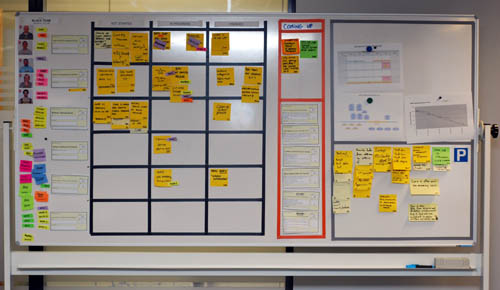
\includegraphics[width=\textwidth]{ScrumWall.jpg}
    \caption{A Scrum Wall. Source: http://www.xqa.com.ar}
	\label{fig:scrum_wall}
\end{figure*}

However, distributed agile teams often use virtual team walls in place of the physical wall so that it is usable across several geographical locations. Figure~\ref{fig:target_process_wall} shows such a virtual wall taken from ScrumPad:

\begin{figure*}[bt]
	\centering
	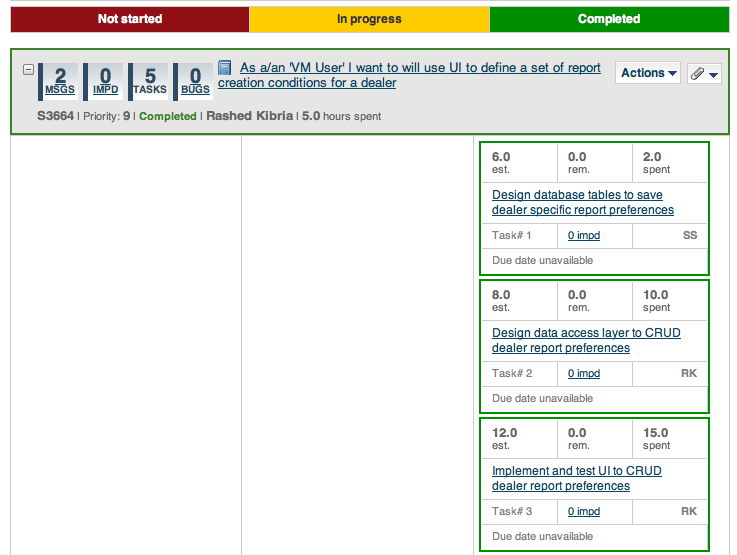
\includegraphics[width=\textwidth]{ScrumPadWall.png}
    \caption{A Virtual Scrum Wall. Source: http://www.scrumpad.com}
	\label{fig:target_process_wall}
\end{figure*}


\section{Distributed Agile Projects}
The members of a distributed agile project work from different geographical locations and adopt agile principles. In practice, the distribution can take several models such as the following three outlined by Braithwaite et al \cite{xp_expanded}:

\begin{enumerate}
	\item Agile outsourcing - the development team is offshore to the customer.
	\item Agile dispersed development - developers spread over different locations, such as open source projects.
	\item Distributed agile development - customers are distributed and one development team is distributed evenly to stay close to the customers.
\end{enumerate}

Again, the geographical distribution can be anywhere between offices across the road to opposite part of the world. For example, a team may work for a customer at the same city or a country separated by ten hours of time zone difference. Distributed agile teams often use different electronic communication channels such as Emails, Instant Messaging, Wiki and Forums as well as online project management tools to uncover the important details about the user stories.

\begin{figure*}[bt]
	\centering
	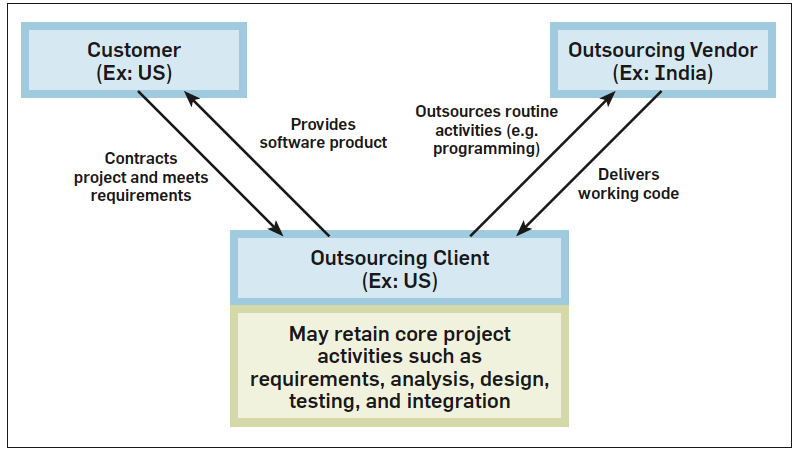
\includegraphics[width=\textwidth]{Distributed.png}
    \caption{An Example Agile Outsourcing Model. Source: \cite{modified_agile}}
	\label{fig:distributed}
\end{figure*}

Figure~\ref{fig:distributed} shows an example of an outsourced agile project taken from \cite{modified_agile}. Similar to this one, a distributed agile project may employ people working on different roles across the globe.

Cost savings has been identified as one of the principal deciding factors for distributing projects across the globe \cite{practical_considerations}. However, projects also go distributed to utilize global talent supply and local knowledge \cite{fully_distributed, modified_agile}. Previous studies have reported success with distributed agile projects. For example, Sutherland et al. reported a linear scalability with a globally distributed outsourced team following a Fully Distributed Scrum (Scrum is a popular agile method) model \cite{fully_distributed}. Similarly, Yahoo! had success with distributed teams that valued people over process and exercised the right information sharing formats and timing \cite{yahoo}.

To ensure a shared view of the ``Product Backlog'' and ``Iteration Backlog'' distributed teams often use web based project management tools. There are a number of such tools available commercially as well as open-source \cite{scrum_pad, version_one, xplanner, trac}. Such tools help people working remotely to have a single backlog and collaborate around that. 

\section{Research Motivation}
The existing literature about collaboration in distributed agile software projects suggest the use of various electronic mediums to counter for missing face-to-face communication. Because of time zone difference, such teams often use asynchronous communication tools such as email and wiki in addition to synchronous ones such as telephone call, instant messaging etc. For example, Robarts \cite{practical_considerations} found that teams would follow up with a written email after they had a telephone meeting to ensure the message is clearly understood. Moreover, of all the available written communication tools, email has been regarded as the most-widely used one by several former studies \cite{collaboration_in} \cite{on_coord}. Additionally, even in collocated settings, people often use emails to communicate as it doesn't require immediate response and overheads like scheduling meetings.

Although having multiple communication channels adds flexibility for collaboration, it also means the knowledge gets fragmented across different channels. This fragmented knowledge may be spread over the project management tool, wiki, emails, instant messages and other places. Basili et al. provided the following list of experiences related to the lack of access to available information \cite{implementing_an_experience}:

\begin{itemize}
	\item An employee left with short notice. The organization lost all of its experience in a certain area and tries to recover it, but it doesn't even know what experience was lost.
	
	\item A consultant spends three weeks developing a course that already exists because he doesn't know that it was done before.
	\item Someone repeats a \$35,000 mistake for which there is a simple solution.
	\item A consultant gave a customer a promise, but is now busy with other work. No one else knows about his promise so it doesn't happen.
	\item An employee learned a lot during a project, but has no time for packaging and dissemination so the knowledge cannot be leveraged.
	\item A new employee is hired, but is for a long time considered a burden instead of help because he needs detailed support from his coworkers, who do not have sufficient time to help him.
	\item (continued...)
\end{itemize}

For agile teams, this situation can be improved with a useful knowledge management solution. To retain the important details about the user stories, one needs to combine these fragmented pieces. But looking into email inboxes of colleagues may be obtrusive to their privacy, if not impossible. Even worse, when a teammate leaves, the emails are gone as well. So, the fragmented pieces of knowledge is either lost or very hard to combine together. Even if one has access to the emails, manually copy-pasting all the emails and combining with the relevant user stories would be a time consuming task to say the least. The following user story and email collaboration shows an example of the knowledge fragmentation:

\begin{quote}
	\textbf{Available in Project Management Tool}\\
	\textbf{User Story}\\
	\textbf{Title:} ``As a/an VM System I want to load Auction data from NADA data file''\\
	\textbf{Description:} Please see the 3 documents related to Auction data
	\begin{enumerate}
		\item Auc Layout
		\item \textbf{Regions Table}
		\item AucData.zip
	\end{enumerate}
\end{quote}

In this example, the user story represents a data integration with a company named NADA. NADA provides vehicle auction information for regions denoted by a ``region code''. However, as the developer starts working on NADA integration, she asks the following question about the region code to the customer through email. 

\begin{quote}
\textbf{Email\#1 (From Developer to Customer)}\\
\textbf{Subject:} ``Initial Questions regarding NADA region value''\\
\textbf{Body:} We found that the Region value can be \textbf{Alpha-numeric} that will be received from NADA Auction. But, the NADA WS accepts only \textbf{Numeric} Region value. Is there any conversion rule to convert the region value into numeric? \\
Thanks
\end{quote}

To answer this question, the customer replies with the following email.

\begin{quote}
\textbf{Email\#2 (From Customer to Developer)}\\
\textbf{Subject:} ``RE: Initial Questions regarding NADA region value''\\
\textbf{Body:} I talked to NADA and they provided me with the \textbf{attached conversion table} for \textbf{Alpha-numeric} to \textbf{Numeric} region codes.
\end{quote}

Please note that the email from the customer included a conversion table for ``region codes''. 

Given this example, if a person only looks at the user story, she will find partial information about it. So, the whole conversion of ``region code''  may be confusing to her. However, when she can see the emails along with the user story, she may have a better understanding about this user story.

This information may be required since a distributed agile team have to cope up with changes in team composition as new people will join and some people may leave. So, if it is possible to combine the fragmented knowledge from different places such as emails, instant messages and project management tools, one can find the important details of the user stories. Such details may not be obvious when only the user story is available. Similarly, the knowledge can help in testing of the features since it is expected to contain customer feedbacks and clarifications on user stories.

The motivation for this thesis stems from the pursuit of developing an agile knowledge base by combining the fragmented knowledge from emails, instant messages and project management tools with the least possible human efforts.

\section{Research Problem}
In software development projects, developers sometimes leave the team for various reasons. As said before, in distributed agile projects, important knowledge is often shared by emails. To transfer this knowledge for future use, one first needs to find the project related emails. Secondly, in such setups people often use web based project management tools to capture user stories and planning information. If the emails can be related to specific user stories in the project management tools, then another developer of the team will be able to easily find the necessary information about a user story when required.

From an end users' point of view, manually finding and relating the emails with user stories is a time-consuming and costly process. This essentially means copying the emails from inbox and putting into a system and linking with a user story. This manual process is cumbersome to say the least. However, if a software can do this, then it may work as a knowledge-base even after someone leaves the team. Such a software needs to be unobtrusive for the most part so that it doesn't require much human effort. So, a technical solution needs to be in place that can capture the project related communication without violating people's privacy. For example, it cannot look into the email inbox of a developer nor should ask a developer to manually enter the chat log into the system.  

The core technical challenge in devising such a software solution is understanding the emails and relating them to specific user stories. The relation between an email and a user story is not explicit. Alternative approaches to make it explicit, such as using identifiable tokens in email subjects, also makes the communication process obtrusive as it adds an extra step to lookup the identity or memorizing it before writing an email. To alleviate this extra step, one can modify email clients to do the lookup. But doing so for the multitude of emails clients including the ones on mobile phones is cumbersome. Also, it imposes a behavioral change or a learning curve for the for the people at the business end.

To find out the implicit relation between a free-format email and a use story, a software needs to handle similarity between two texts, which is a standard problem. Emails may not show very high text similarity with the related user stories. This text component makes the relevance between a user story and an email an approximation or fuzzy match. Also, pure text retrieval limits how accurate the assignment of email and user stories can be. This is because people use different vocabulary and often a tacit communication is there underneath a written form. Using context information has the potential to increase this accuracy. So, a software needs to be able to combine both the text and context similarity for auto-tagging emails with user stories.

To account for the context, one needs to use the associated meta information that are available. The contexts of an email and a user story are not exactly similar. For example, the context of an email has a time-stamp, sender, recipients and past conversations. On the other hand, user stories have a different context, such as their development time or iteration timeframe, developers and customers. An auto-tagging solution needs to use these context meaningfully so that each component gets its deserving share of importance in the relevance computation. So, it is important to have a formula that produces similarity ranking considering the fuzzy text similarity and associated context relevance.

Next technical challenge is to evaluate the accuracy of the auto-tagging system. For the auto-tagging to be useful, it shouldn't make too many mistakes in finding similarity. The accuracy of this system needs to be tested using real world data. 

Another technical challenge is to design an adaptive auto-tagging system so that it can adapt to different communication patterns. Since distributed agile teams across the world have differences in who, how and when they communicate about their user stories, the auto-tagging system needs to adjust its similarity computation accordingly. For example, one team might spend more time communicating about user stories that are currently under development while another team might prefer to discuss about the upcoming ones. An auto-tagging system that uses the meta information of time needs to learn this pattern to make a right decision.


\section{Research Goals}
\begin{figure*}[bt]
	\centering
	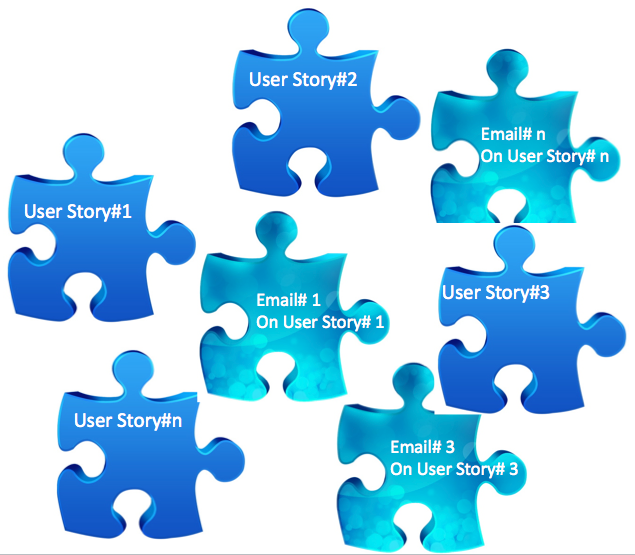
\includegraphics[width=\textwidth]{Jigsaw.png}
    \caption{Jigsaw Puzzle Visualizing the Auto-Tagging Problem}
	\label{fig:jigsaw}
\end{figure*}

The principal goal of this research is to develop a tool that can automatically read and relate emails with user stories based on agile project context. The tool needs to minimize human efforts in doing so. Another complementary goal is to evaluate the tool using real world data. The underlying approach and evaluation of Taggy is discussed in Chapters ~\ref{ch:taggy} and ~\ref{ch:evaluation}.

Figure~\ref{fig:jigsaw} visualizes the research goal as it shows the fragmented knowledge from project management tools and email inboxes to be combined in a jigsaw puzzle. The target is to solve this puzzle so that each user story gets connected to the relevant project related emails.

This research also aimed to investigate the difficulties in solving the various aspects of the research problem, namely i) relevance ranking of user stories for a given email, ii) using text similarity in addition to context relevance, iii) evaluating auto-tagging accuracy and iv) developing an adaptive auto-tagger. The findings from this investigation is expected to provide a foundation for next level of research in this area.

\section{Key Contributions}
This research work has been published and presented at XP 2010 \cite{auto_tagging}. 

The key contribution of this research is, it demonstrates a novel approach of building a knowledge-base for distributed agile teams from emails and user stories. This approach has the similar motivation as found in some previous works, such as clustering emails archives\cite{using_hybrid}, tagging forum messages with source code change set\cite{hipikat, hipikat_2} and using wiki to share knowledge. However, this research shows a machine learning approach to conglomerate fragmented knowledge from emails, instant messages and project management tools minimizing human efforts. This new technique adds to the existing body of knowledge.
                                  
Another key contribution is, it shows that text and context similarity can be used to find relevance between two different types of entities such as emails and user stories, where the degree of text similarity may be inadequate. We have used Case Based Reasoning (CBR) for auto-tagging. As this research findings suggest, other CBR systems concerning different entities may utilize this technique.

\fancyhead[RO,LE]{\thepage}
\fancyfoot{} 
\chapter{LITERATURE REVIEW}
Researchers have attempted to solve the problem of knowledge management for software development projects from different points of view. Also, the industry is using a number of available commercial and open-source tools to retain and manage knowledge. To find the similarity and contrast of this research with the existing approaches, this related work chapter is divided into sections dedicated to the following five areas:

\begin{enumerate}
	\item Communication in distributed teams
	\item Capturing knowledge from emails
	\item Wiki based knowledge sharing
	\item Context based knowledge management
	\item Review of existing tool support for knowledge sharing
\end{enumerate}

\section{Communication in Distributed Teams}
The Agile Manifesto\cite{agile_manifesto} puts heavy emphasis on customer collaboration. Understandably in distributed projects, the geographical and temporal distance accounts for communication challenges compared to a collocated setup. Several existing research focused on the use and effectiveness of the different communication channels that are used in distributed projects.

Thissen et al. points out that a distributed team to become successful must use appropriate tools to ensure easy flow of information \cite{communication_tools}. Lanubile provided a categorization of such collaboration tools \cite{communication_in_distributed} that include software configuration management, bug and change tracking, build and release management, product and process modeling, knowledge center and communication tools. Lanubile also pointed out that asynchronous communication tools include emails, mailing lists, newsgroups, web forums and blogs while synchronous ones include telephone and conference calls, chat and video conferencing. Of all the asynchronous tools, email has been identified as the most widely-used and successful collaborative application because of its flexibility and ease of use.

The use of synchronous vs. asynchronous mediums depends on teams and their temporal as well as geographical distance. For example, Hole et al. found that teams often preferred email and chat over telephone calls for meeting between two sub-teams at two different locations due to language barriers \cite{a_case_study_of}. Here is an excerpt from a Scrum Master, one of the participants of their study:\\
\emph{``we tried to use telephone conferences, but it did not work well, because of language problems. It is also easier to understand each other when relying on written communication. Also extensive use of chatting makes it possible to ask a question right away. It takes time to organize a telephone-conference.''}

Korkala et al. found that despite the availability of richer communication media, the customers preferred to use emails for most of their mid-iteration communication needs\cite{korkala}. Here is an opinion from a customer of their case study about the selection of mid-iteration communication:\\
\emph{``Emails will do just fine. They are enough.''}

Hildenbrand et al. suggested that customers and testers of distributed agile teams need to work closely to flesh out the acceptance criteria for the user stories in the iteration backlog \cite{agile_methods}. Also quick feedback from the customers is needed during the design and development of a user story. They also emphasized that this knowledge could be of great use and must be shared with the whole team. To collaborate and capture this knowledge, they suggested the use of online groupware and instant messaging.

Cataldo et al. looked into the types of knowledge contained in the emails of a distributed project and found that email was the most preferred medium for information exchange and task negotiation related topics\cite{on_coordination}. Although the target was to use groupware for such activities so that the knowledge could be easily retained shared, their data suggests that developers relied heavily on emails for information acquisition. Layman et al. classified the emails exchanged in a distributed agile project into several types such as: i) Changes in specification, ii) Clarification, iii) Prototype, iv) Feedback, v) Planning/scope, vi) Bug, vii) Acceptance test and viii) Post-release bug related emails \cite{essential_communication}. They also found that clarification related emails were the most frequently exchanged of all these categories.

To summarize, this section of the literature review suggests that distributed teams often use emails and other text-based asynchronous mediums alongside real-time collaboration tools to share important knowledge about their projects. Based on these findings, this thesis emphasized on automatically capturing project related emails and instant messages. Since emails and instant messages are widely-used to share knowledge among people in distributed projects, the solution shown in this thesis can be used to retain and reuse this knowledge.

\section{Capturing Knowledge from Emails}
In the existing literature, there have been attempts to extract knowledge by mining software project related emails. Largely, the concentration of such mining efforts has been around clustering the archives to meaningful groups. Also, there has been work around the visualization of email archives so that one can easily navigate the corpus of emails.

Berlin et al. designed and implemented a group memory system called TeamInfo \cite{where_did_you}. TeamInfo let people to use CC: or carbon copy feature of emails to forward a project related email to the TeamInfo system. Once TeamInfo reads the email, it finds the predecessors if any and try to classify the email into one of the preset categories. These preset categories are similar to what we see in email folders or filters, namely grouping by one or more of conditions involving sender, recipients, subject and text containment. This classification is intended to help in browsing the emails based on their high level categorization. However, they faced challenges with coming up with categorizing conditions as at times one email could be part of multiple categories. Also, a fine grained categorization would lead to hundreds of such classes, which again, makes it hard to easily browse to a topic of interest. To write a filter, TeamInfo required significant experience as the rules were expressed using a declarative language. TeamInfo helped them in retaining and sharing knowledge. Taggy has a similarity with the data feed process of TeamInfo, as it uses the same CC: feature of emails to get hold of the knowledge. However, Taggy is designed to help agile teams, where the presence of assigned developers, customers and time box provide a context to the plain text-based user stories. As a result, instead of trying to group the emails, Taggy tries to automatically link up emails with the user stories so that one can follow the discussions related to specific features of a software. This alleviates the overhead of creating and managing shared grouping rules.

A knowledge-base is often used to recommend a developer about required source code change locations. Hipikat is such a recommender that uses interlinked information from several sources, such as CVS log messages, online documents and newsgroup threads\cite{hipikat}. Here, the newsgroup threads are essentially the group emails exchanged among people working on a project. To infer the relationship between a thread discussion and other artifacts, Hipikat uses ``References'', a header element that can identify the thread's topics of interest. However, in agile projects such email threads are often exchanged between customer and developers and it might require extra effort either to memorize or to lookup the ``References'' identity every time before starting a discussion. Taggy emphasizes seamless customer collaboration and reduces this extra look up cost through utilizing machine learning techniques to infer the hidden relation between an email and user story.

Existing research also looked into mining and visualizing the contents of software related email archives to extract out the important patterns. For example, Medynskiy provided a multi-modal visualization of email, instant message and CVS commit logs from the Python project\cite{using_hybrid}. They mined the text information to extract out meaningful groups and interlinked among the groups to contributors of the contents. This way, one could navigate related knowledge from different sources that are otherwise fragmented. In effect, Taggy also tries to unite the fragmented pieces of information. But the concentration is at a higher level (user stories) as opposed to lower level artifacts (CVS logs). Also, instead of mining the archived data sources, Taggy builds the knowledge-base on the go.

Software requirements traceability helps understanding a requirement based on its underlying reasoning\cite{requirment_traceability}. However, for distributed agile projects, this is hard since knowledge is dispersed. Capturing the emails with user stories has the potential to improve the traceability in such cases. To attain this goal, the approach of Taggy is in alignment with the aforementioned research about building a knowledge-base from emails. However, it is extended to be used in agile projects, where the use of available context helps the computer to make an informed guess about if an email is related to a user story or not.

\section{Wiki Based Knowledge Sharing}
The overwhelming success of Wikipedia \cite{wikipedia} is a result of collaborative editing. Being inspired by this, several researchers explored the potential of using Wiki for software knowledge management. For example, Decker et al. have found successful requirement capturing and stakeholder participation through wiki platform\cite{wiki_based}. They proposed a document structure or template for using Wiki in software projects so that different artifacts such as user stories, tasks and plans can be managed following a standard approach. However, they also discovered that using wiki for such tasks adds complexity resulting from its syntax to denominate metadata.

Decker et al. also proposes the use of semantic wiki, an approach where additional meta information is used, so that it is possible to reuse the contents using machine learning \cite{self_organized}. In this regard they introduced Wikitology, a term that combines Wiki and Ontology. The Ontology is contained as a part of meta-data in the templates for different software engineering artifacts, such as user stories, discussions etc. Once these templates are defined, a software engineering artifact becomes an instance of one of the templates. So, the relationship between two different wiki pages can be established based on their underlying templates' meta information. Given the ontology of different wiki pages, they used two techniques, Latent Semantic Analysis and Case Based Reasoning, to compute the similarity. In this thesis I used the second technique, CBR, to find similarity between an email and a user story. However, instead of using a predefined ontology, Taggy uses the available meta information or context from an email. Also, Taggy combines the context and text similarity in the computation as opposed to solely relying on the context.

Tosic et al. developed a Collaborative Semantic Web Portal Prototype that utilizes wiki platform for collaborative knowledge acquisition to be used in agile project management \cite{collaborative_knowledge}. Their solution added access control to the wiki pages and also several indicators such as number of contributors, the creator and so on for every page. Using this system they observed encouraging results such as teamwork and collaboration, open information flow and the light-weight agile vigilance. 

To ease the authoring of wiki pages, OntoWiki shows a few interesting techniques \cite{ontowiki}. For example, they present a rich editor with support for real-time search from existing content to reduce the time required to produce an article and cross-link with different pages. Also, to make it collaborative they brought the concept of commenting and rating. While these techniques can greatly help in authoring wiki content, to be used in software knowledge management, the developers and the customer need to actually put the contents on the wiki and ensure the contents are updated accordingly. This may be a barrier, as it requires considerable human efforts to a cause that have lower immediate business value compared to some other tasks, such as developing and testing the software.

Chau et al. studied the contribution to a software wiki contents from people working on different roles \cite{a_case_study_of_wiki}. They observed the use of MASE, a wiki-based knowledge sharing system, in a medium-sized software company. They discovered a very high usage, exceeding 90\%, of MASE as an asynchronous collaboration medium. But surprisingly, only 10\% of the wiki content were produced by the managers, while the rest was contributed by the technical team. Moreover, none of the managers were in the list of top 10 contributors. They also found that there was a greater need for unstructured than structured knowledge. In agile software engineering, informal and continuous customer collaboration is heavily utilized. So, it is important to choose a knowledge sharing media that offers most flexibility as well as less learning curve for the customers. This thesis recognizes the need for unstructured knowledge and uses email as a source of such knowledge. As a result, the knowledge base is generated while people communicate as opposed to ``documented after the knowledge is shared''.

Wiki has also been used to write executable acceptance tests with the motivation that customers can provide the acceptance criteria for a user story in simple wiki tables \cite{fitnesse}. For example, Young et al. mentioned the use of wiki for automated acceptance tests so that the continuous integration system could execute the tests\cite{how_did_we}. However, such tabulation of acceptance tests often do not capture the underlying knowledge behind the facts, which may be necessary to understand a user story.

While wiki can work as a knowledge sharing tool, an addition of email discussions offer several unique benefits. For example, email is a general purpose communication tool, so most people are already familiar with this. Wiki is great for collaborative editing. But knowledge sharing often takes the form of discussion where information flows back and forth between people. For example, it is easy to follow a discussion than to find the latest changes in a  wiki page. As Chau et al. pointed, wiki and similar centralized knowledge capturing approach often employs people who are not involved in the day-to-day software development and as a result, there are concerns raised about the usefulness of this approach\cite{a_case_study_of_wiki}. Capturing knowledge from emails and linking them with user stories will complement the collaborative editing benefits of wiki. So, it will bring the useful details that are already discussed from emails and add to the knowledge from the wiki, if any.

\section{Context Based Knowledge Management}
Maalej et al. provided a context based solution for lightweight knowledge sharing in distributed software projects \cite{a_lightweight}. They identified two key steps in the knowledge sharing process, namely, knowledge access and knowledge sharing. They outlined a framework to facilitate the access to relevant implicit knowledge from the large amount of dispersed sources. The framework relies on the context of different knowledge items as well as knowledge consumer's usage pattern to proactively provide access to the available knowledge. To facilitate knowledge sharing, they identified that a knowledge provider needs to present the knowledge in generalized format so that it can be applied on a different context by another person. This requires additional efforts from the provider without much of an immediate benefit.

To minimize this burden, they proposed the use of additional semantic information or ontology in knowledge items, which can be used in computer-based information retrieval through context matching. Their proposed knowledge management solution derives a profile of the developers from their usage history. Based on this profile and the semantic information present at the knowledge items, the relevant ones are found. This proposed solution mainly targets the knowledge capturing at a fragment of source code level. Although this framework provides an abstract form for a knowledge management solution, a concrete description of how the acquisition of dispersed knowledge from sources like emails, wiki, instant messages and forums are incorporated is not discussed. As suggested in this approach, Taggy uses the context information in addition to text relevance to interlink different knowledge items. However, Taggy is designed to capture high level knowledge from emails and user stories as opposed to the level of source code fragments.

Ratanotayanon et al. developed Zelda, an Integrated Development Environment (IDE) plugin to interlink source code with user stories \cite{supporting_program}. This plugin provides an interface where a developer can select one of the user stories as an active user story. Next, when she is ready to push the changes in the code repository, the plugin automatically links all the changes against the active user story. It also allows a developer to manually select source code that are related to the user story. The goal of this link recording is to help other developers who might need to make changes to the feature from an existing user story. To complete the future modification, one can navigate to relevant source code from the stored links. Since it is a common practice to modify source code and keep revisions, Zelda updates the user story and code links whenever the code has a new revision to keep the links pointed to the latest revision. In their evaluation, they found that Zelda helped developers to focus on relevant source files given a new user story to modify an existing one.

The concept behind Zelda, linking source code changes with requirements and other high level artifacts, is also present in FEAT\cite{feat} and Mylyn\cite{mylyn}. For example, Mylyn is an IDE plugin that builds a task context as developers select a task and make necessary changes. The context of a task includes information about the source code changes, API usage and documentation lookup as a developer works on it. Having this context, a developer can easily navigate and search though relevant source code for a task. Mylyn also has integrations with several task and bug tracking tools.

As seen with Zelda and Mylyn, high level artifacts such as user stories and tasks can be used as an entry point to a knowledge base. Taggy follows this same approach. However, instead of linking the source code with the user stories, Taggy links the email discussions. So, the knowledge base produced by Taggy is likely to complement Zelda with relevant higher level information from emails that can provide more insights into the user stories. In a sense, Taggy interlinks two high level artifacts which complements the knowledge found from the interlinked low level items.

\section{Review of Existing Tool Support for Knowledge Sharing}
Distributed agile projects often use globally available project management tools to share knowledge \cite{essential_communication}. These tools allow the teams to capture the product and iteration backlogs, user stories and project planning information. Typical project planning information includes the estimation and assignment of tasks or user stories to developers and testers. Also, some tools provide support for collaboration about the user stories.

There are a number of commercial tools available for agile project management such as VersionOne\cite{version_one}, Mingle\cite{mingle}, ScrumPad\cite{scrum_pad}, ScrumWorks\cite{scrum_works}, IBM Rational Team Concert\cite{ibm_rtc} etc. These tools offer templates for capturing various agile software engineering artifacts such as user stories, backlogs, acceptance tests and so on. Also, they provide process specific workflows, for example, a workflow for Scrum includes a virtual story wall, burndown and other charts for distributed project tracking. Some of these tools let people to collaborate using message threads and wiki. These tools are generally useful in planning and tracking activities. In addition to commercial tools, one can also use open-source agile project management tools such as XPlanner\cite{xplanner} and Trac\cite{trac}.

Several issue or bug tracking tools such as Jira\cite{jira}, Bugzilla\cite{bugzilla}, FogBugz\cite{fog_bugz} are being used in distributed agile projects as well. To support agile processes, these tools offer plugins for agile projects that include some of the features from the aforementioned project management tools. These bug tracking tools provide a messaging system where people can collaborate around bugs. The knowledge shared during this collaboration is often used to solve new bugs\cite{issue_tracking}.

Distributed agile teams often use general purpose project management tools such as Basecamp\cite{basecamp}, Teambox\cite{team_box} etc. While these tools are not tailored to provide agile specific artifacts, they are often picked for their simplicity to use. So, instead of providing a template for an user story or an issue, this tools simply provide a to-do list. Similarly, instead of iterations, people rely on milestones. And as seen with other tools, the general purpose web-based project management tools also allow people to use messaging systems to collaborate on their to-do lists.

Alongside project management tools, some distributed agile teams use general purpose shareware tools such as Microsoft SharePoint\cite{share_point}. SharePoint provides an infrastructure to manage websites, communities, content, search and reporting that is mainly configuration based and does not require coding efforts for the most part. In large distributed agile projects, where multiple teams are involved, SharePoint is often used to manage the knowledge.

Some agile projects are now using source code hosting platforms for project management as well. For example, github\cite{github}, CodePlex\cite{codeplex} and similar source code hosting platforms have support for defining issues and user stories. Also, they allow some project planning features such as iteration backlogs, estimation and assignment of work items etc.

Agile teams also use continuous integration tools such as Hudson\cite{Hudson}, CruiseControl\cite{cruise_control}, Microsoft Team Server\cite{team_server} etc. so that the status of the current build is automatically communicated. These tools provide a dashboard and detail view of a project's health that include build stats, test results and commit history. Distributed agile teams often use a separate tool capture knowledge about the high level artifacts that are not found in the continuous integration tools.

The aforementioned tools help the distributed agile teams to collaborate and share project related knowledge. Almost all of them send out notification emails when a change takes place. For example, when a user story is assigned or a build succeeds. Such email notification is helpful since it reaches the inbox of people instead of waiting for them to visit the tools. Some of the tools, such as Basecamp, FogBugz etc. also accept incoming emails from people. But none of the the tools interlinks the incoming emails to the user stories unless a user does it manually. As a result, the benefits of a message thread attached to a user story is not readily available. To ensure the message threads are kept attached to the user stories, the users are forced to use the tools. But, similar to email notification, this could be convenient if a developer or a customer could just send an email to the tool and the tool would automatically attach the email to the relevant user story. Taggy attempts to solve this problem by utilizing the planning information from the project management tools to infer the relevance of an user story against an email.
%\include{chapter3}
%\include{chapter4}
%\include{chapter5}
% \appendix
% %!TEX root = /Users/smsohan/Taggy/Thesis/ucalgthes1_root_0.tex
\fancyhead[RO,LE]{\thepage}
\fancyfoot{} 
\chapter{Ethics Approval}

The ethics approval for conducting the qualitative evaluation of Taggy is given at Figure~\ref{fig:ethics}:

\begin{figure*}[bt]
	\centering
	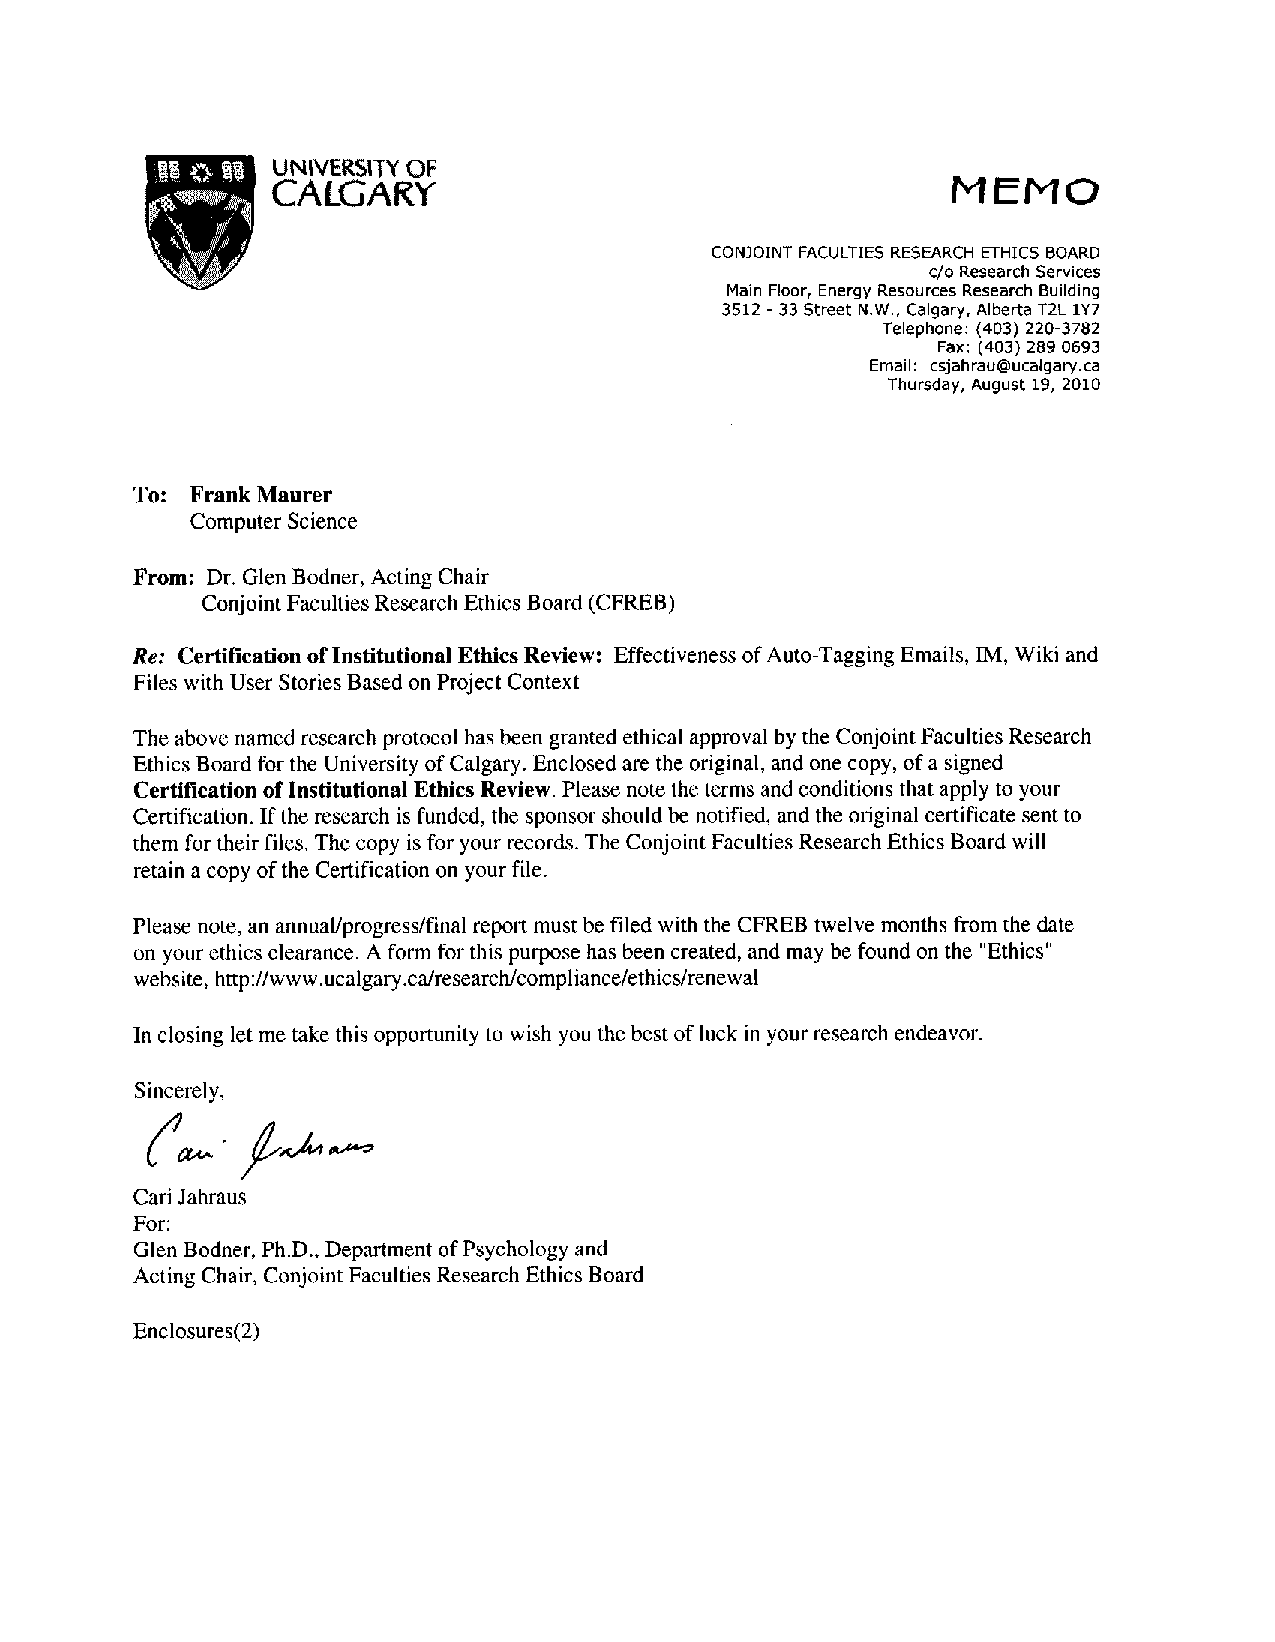
\includegraphics[width=\textwidth]{ethics.pdf}
    \caption{Ethics Approval}
	\label{fig:ethics}
\end{figure*}




\end{document}
